\documentclass{article}
  \usepackage[total={18cm,21cm},top=2cm, left=2cm]{geometry}
  %Paquetes adicionales
  \usepackage{latexsym,amsmath,amssymb,amsfonts}
  \usepackage[latin1]{inputenc}
  %\usepackage{txfonts}
  \usepackage[T1]{fontenc}\usepackage{ae,aecompl}
  \usepackage{graphicx}
  \usepackage[usenames]{color}
  \usepackage[spanish]{babel} % Idioma espa�ol
  \usepackage{tcolorbox}
\usepackage{multirow}
\tcbuselibrary{theorems}
  %---------------comandos especiales-------------------------------
  \newcommand{\R}{\mathbb{R}}
  \newcommand{\Z}{\mathbb{Z}}
  \newcommand{\Q}{\mathbb{Q}}
  \newcommand{\C}{\mathbb{C}}
  \newcommand{\N}{\mathbb{N}}
  \newcommand{\I}{\mathbb{I}}
  \newcommand{\F}{\mathbb{F}}
  
 
% Definindo novas cores
\definecolor{verde}{rgb}{0.25,0.5,0.35}
\definecolor{jpurple}{rgb}{0.5,0,0.35}
\definecolor{darkgreen}{rgb}{0.0, 0.2, 0.13}
%\definecolor{oldmauve}{rgb}{0.4, 0.19, 0.28}
% Configurando layout para mostrar codigos Java
\usepackage{listings} %-----------------------------------------------------------------

\lstdefinelanguage
   [x64]{Assembler}     % add a "x64" dialect of Assembler
   [x86masm]{Assembler} % based on the "x86masm" dialect
   % with these extra keywords:
   {morekeywords={JMZ,LOD,STO,JMP,ADD,DIV,HLT, %
                  POPFQ,PUSHFQ,SCASQ,STOSQ,IRETQ,RDTSCP,SWAPGS, %
                  rax,rdx,rcx,rbx,rsi,rdi,rsp,rbp, %
                  r8,r8d,r8w,r8b,r9,r9d,r9w,r9b, %
                  r10,r10d,r10w,r10b,r11,r11d,r11w,r11b, %
                  r12,r12d,r12w,r12b,r13,r13d,r13w,r13b, %
                  r14,r14d,r14w,r14b,r15,r15d,r15w,r15b}} % etc.

\lstset{language=[x64]Assembler}

\newcommand{\estiloJava}{
\lstset{
    basicstyle=\ttfamily\small,
    keywordstyle=\color{jpurple}\bfseries,
    stringstyle=\color{red},
    commentstyle=\color{verde},
    morecomment=[s][\color{blue}]{/**}{*/},
    extendedchars=true,
    showspaces=false,
    showstringspaces=false,
    numbers=left,
    numberstyle=\tiny,
    breaklines=true,
    backgroundcolor=\color{cyan!10},
    breakautoindent=true,
    captionpos=b,
    xleftmargin=0pt,
    tabsize=2
}}


\definecolor{ceruleanblue}{rgb}{0.16, 0.32, 0.75}
\usepackage{fancyhdr}
\pagestyle{fancy}

\begin{document}

Un tanque en forma de cono circular recto de altura $H$ radio $R$ y v�rtice debajo de la base, esta totalmente lleno con agua.\\
Determine el riempo de vaciado total si $H=12$ pies, $R=5$ pies, $a=1$pulg$^2$ y $C=0.6$

\begin{center}
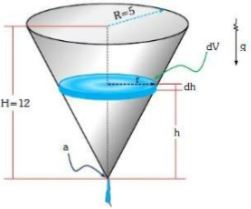
\includegraphics[scale=1]{c1}
\end{center}

$$A(h)\frac{dh}{dt} = ac\sqrt{2gh}$$

Como las dimensiones de el tanque esta en pies se pasa el valor de $a$ a pies.
\begin{align*}
a &= 1 \,\mathrm{pulg}^2\\
a &= (1/12)^2 \,\mathrm{pies}^2\\
a &= 1/44\,\,\mathrm{pies}^2
\end{align*}

Como se puede ver en la figura la secci�n transversal son circunferencias de radio $r$, con $r$ variable.
$$A(r) = \pi r^2$$

Ahora se ocupa dejar $r$ en funci�n de $h$ mediante igualdad de triangulos.

\begin{center}
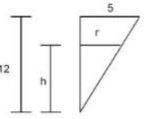
\includegraphics[scale=1]{c2}
\end{center}
\begin{align*}
\frac{r}{h} &= \frac{5}{12}\\
r &= \frac{5h}{12}
\end{align*}
Con esto sustituimos en $A$
\begin{align*}
A(h) &= \pi \left( \frac{5h}{12} \right)^2\\
A(h) &= \frac{25\pi h^2}{144}
\end{align*}

Con esto sustituimos:
\begin{align*}
\frac{25\pi h^2}{144}dh = -\frac{1}{144}(0.6)\sqrt{64h}dt
\end{align*}
Ac� se construye la ecuaci�n diferencial asociada.\\
\begin{align*}
25\pi h^2 dh = -4.8\sqrt{h}dt\\
25\pi h^{3/2} dh = -4.8dt\\
\int25\pi h^{3/2} dh =\int -4.8dt\\
10\pi h^{5/2}  = -4.8t + C\\
\end{align*}
Luego tenemos las condiciones para calcular el valor de $C$
\begin{align*}
10\pi (12)^{5/2}  &= -4.8(0) + C\\
C &= \frac{25\pi (12)^{5/2}}{12} 
\end{align*}
Simplificando en la expresi�n y despejando el valor de $h$ tenemos.
\begin{align*}
10\pi h^{5/2} &= \frac{25\pi (12)^{5/2}}{12} - 4.8t\\
h(t)  &= \left( 12^{5/2} - \frac{12}{25\pi}t \right)^{2/5}
\end{align*}
Por ultimo para determinar el valor del tiempo total del vaciado $t$ eso ocurre cuando $h=0$ 
\begin{align*}
0  &= \left( 12^{5/2} - \frac{12}{25\pi}t \right)^{2/5}\\
t &= \frac{25\pi(12)^{5/2}}{12}\\
t&= 3264.83 \,\,\mathrm{s}
\end{align*}
Por lo tanto el tanque se vac�a en 3264.83 segundo o 54,25 min.
\end{document}
